\chapter{Complete Feature List}
\label{ch:features}

\section{User Authentication \& Authorization}
\label{sec:auth-features}

\textbf{Workflow:}
\begin{enumerate}[leftmargin=*,topsep=3pt,itemsep=2pt]
    \item User visits login page and chooses authentication method (Email/Password or OAuth)
    \item For OAuth: Redirects to provider (Google/GitHub), returns with authentication token
    \item Backend validates credentials, generates JWT token with RS256 encryption
    \item Session stored in database with 30-day expiry, user redirected to dashboard
\end{enumerate}

\textbf{Database Tables:} \texttt{User}, \texttt{Account}, \texttt{Session}, \texttt{VerificationToken}

\begin{figure}[H]
\centering

\includegraphics[width=0.7\textwidth]{images/screenshots/sign_in.png}
\caption{Authentication Interface}
\label{fig:auth}
\end{figure}

\section{Paper Annotation \& Highlights}

    \textbf{Workflow:}
\begin{enumerate}[leftmargin=*,topsep=3pt,itemsep=2pt]
    \item Open a paper and select text to create a highlight or note
    \item Add a short comment; annotations are stored and scoped to user/workspace
    \item Toggle filters to view all notes, only mine, or team highlights
    \item Annotations appear contextually when revisiting the paper
\end{enumerate}

    \textbf{Database Tables:} \texttt{Annotation}, \texttt{Note}

\begin{figure}[H]
\centering
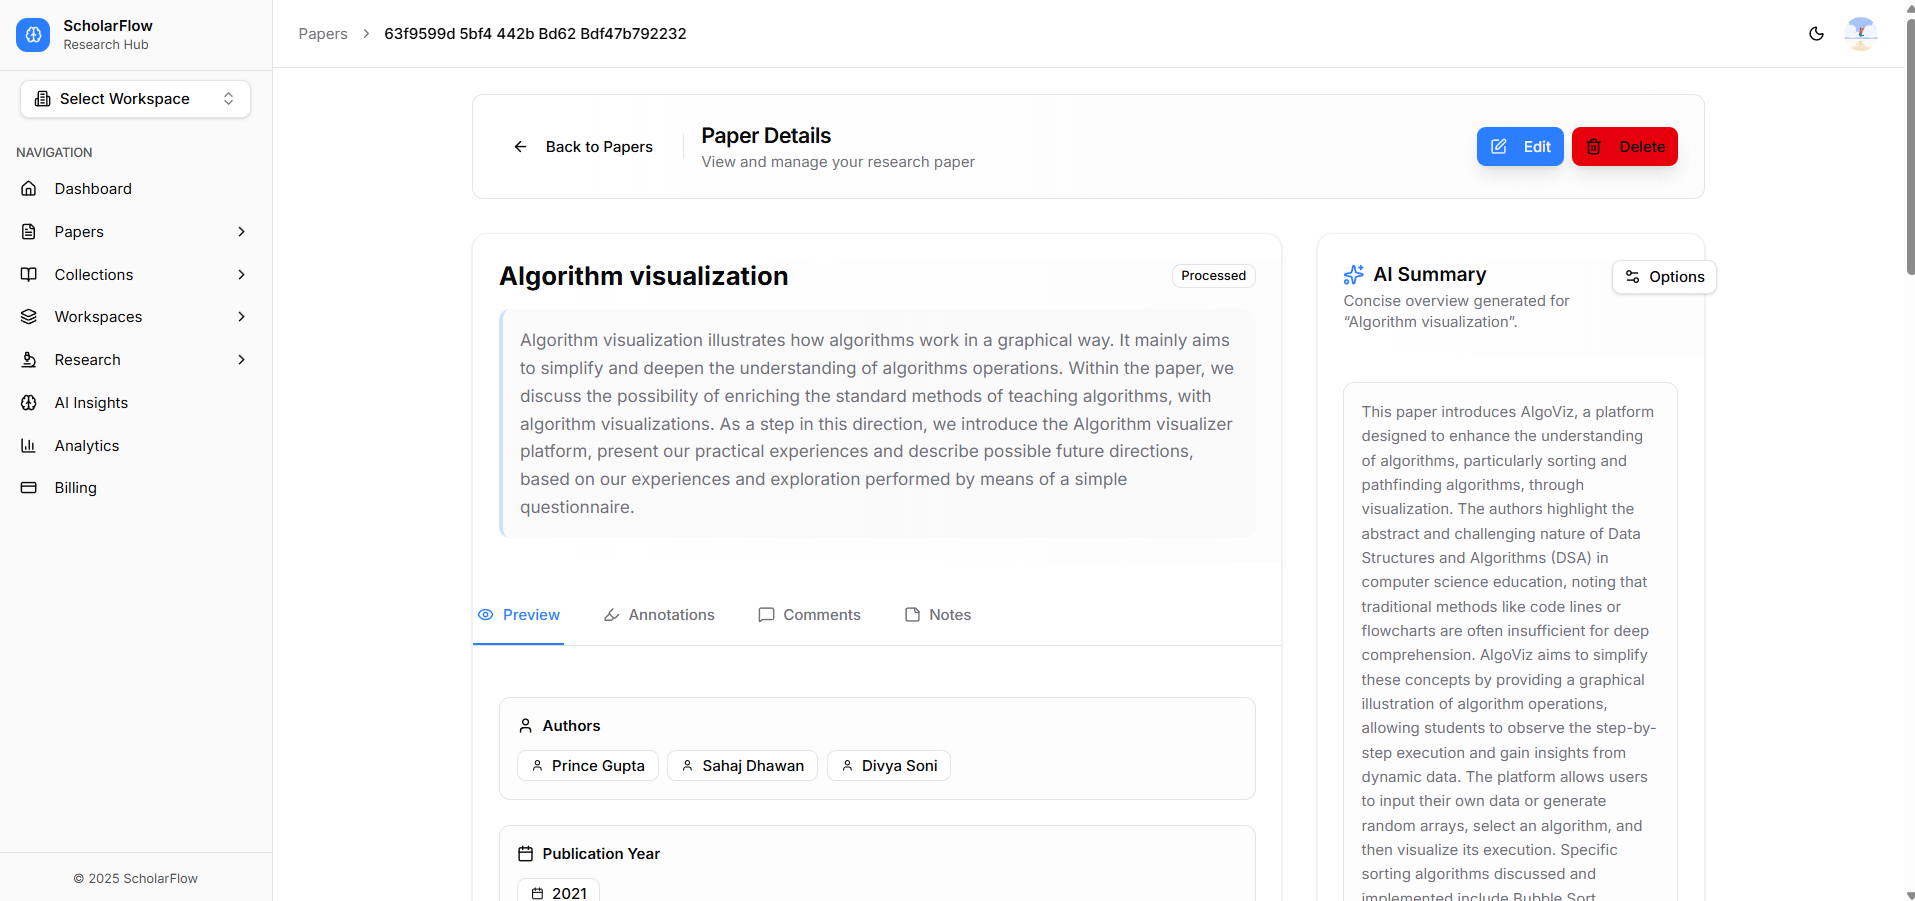
\includegraphics[width=0.8\textwidth]{images/screenshots/paper_details_1.png}
\caption{Inline Annotations on Paper}
\label{fig:annotations}
\end{figure}

\section{Notifications \& Email Invitations}

    \textbf{Workflow:}
\begin{enumerate}[leftmargin=*,topsep=3pt,itemsep=2pt]
    \item Team lead invites a member to a workspace or shared collection
    \item Email is sent with a secure link; pending invites are tracked
    \item In-app notifications summarize membership changes and comments
    \item Users can accept/decline and manage notifications from settings
\end{enumerate}

	\textbf{Database Tables:} \texttt{WorkspaceInvitation}, \texttt{Notification}

\begin{figure}[H]
\centering
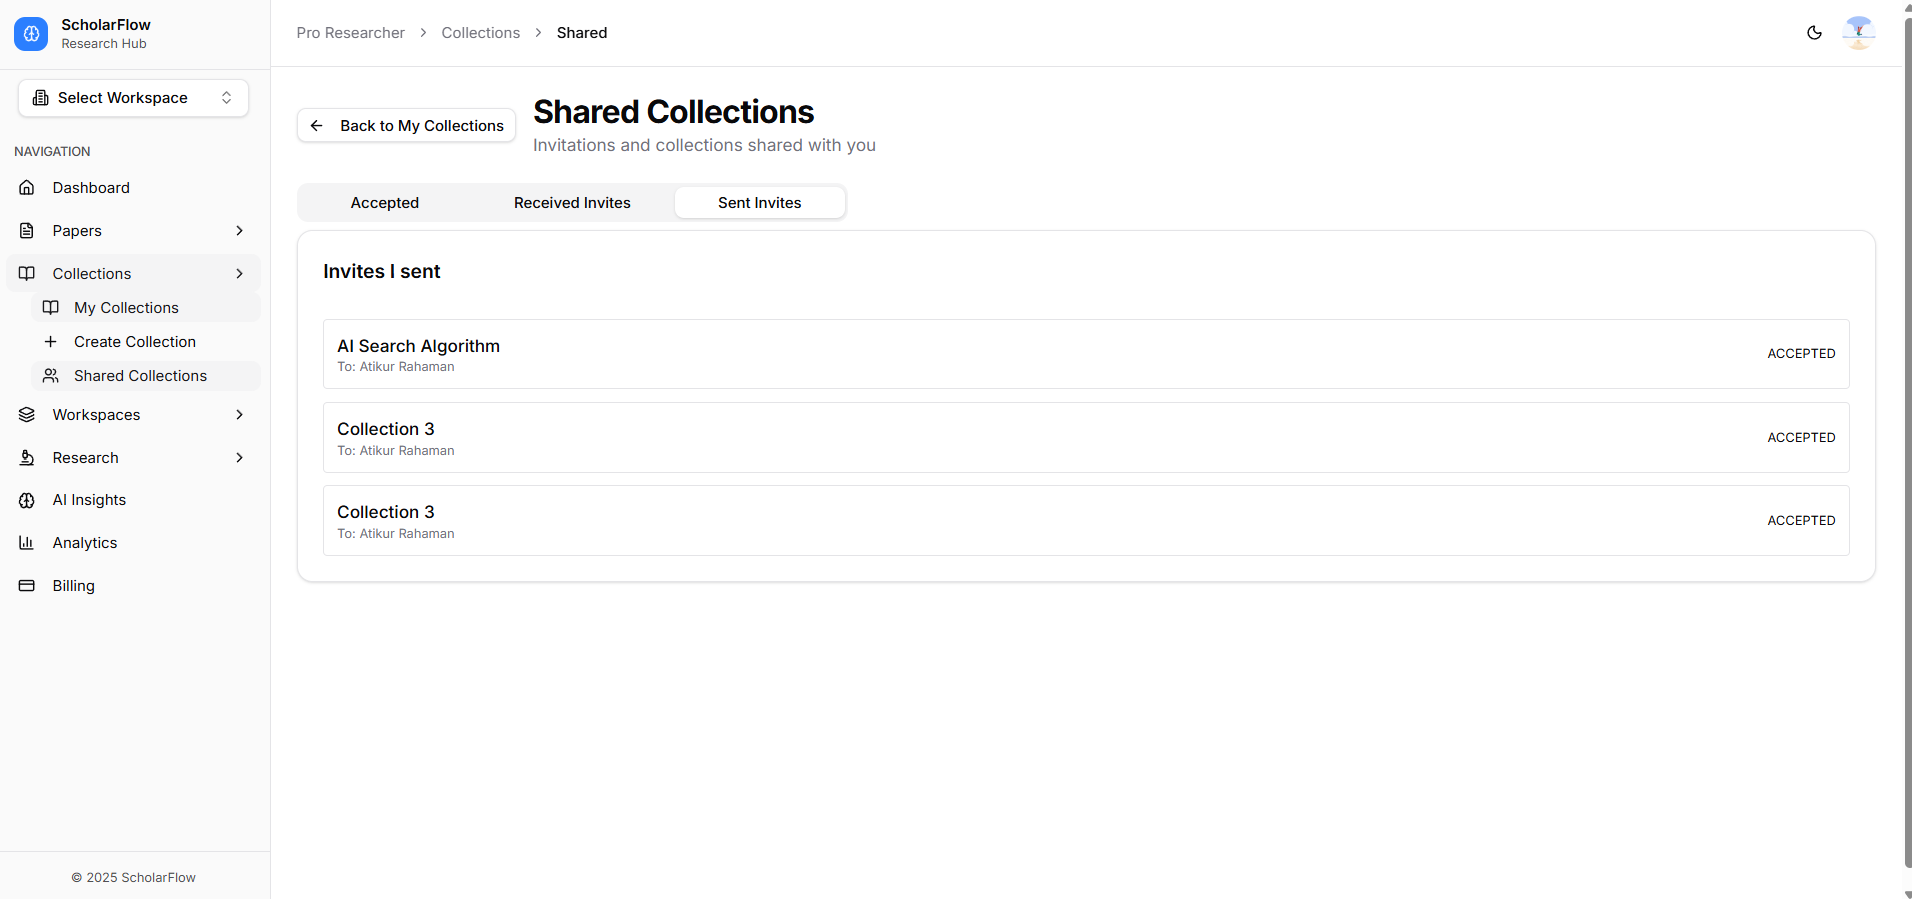
\includegraphics[width=0.75\textwidth]{images/screenshots/shared_collection.png}
\caption{Sharing \& Invitations}
\label{fig:notifications}
\end{figure}

\section{Paper Upload \& Management}

\textbf{Workflow:}
\begin{enumerate}[leftmargin=*,topsep=3pt,itemsep=2pt]
    \item User drags PDF/DOCX file to upload area (max 25MB)
    \item Frontend generates presigned S3 URL, uploads directly to AWS S3
    \item Backend extracts metadata (title, authors, abstract) using PDF parser
    \item Text chunked into segments for AI processing, stored in \texttt{PaperChunk}
    \item Paper listed in user's workspace with searchable metadata
\end{enumerate}

\textbf{Database Tables:} \texttt{Paper}, \texttt{PaperFile}, \texttt{PaperChunk}

\begin{figure}[H]
\centering
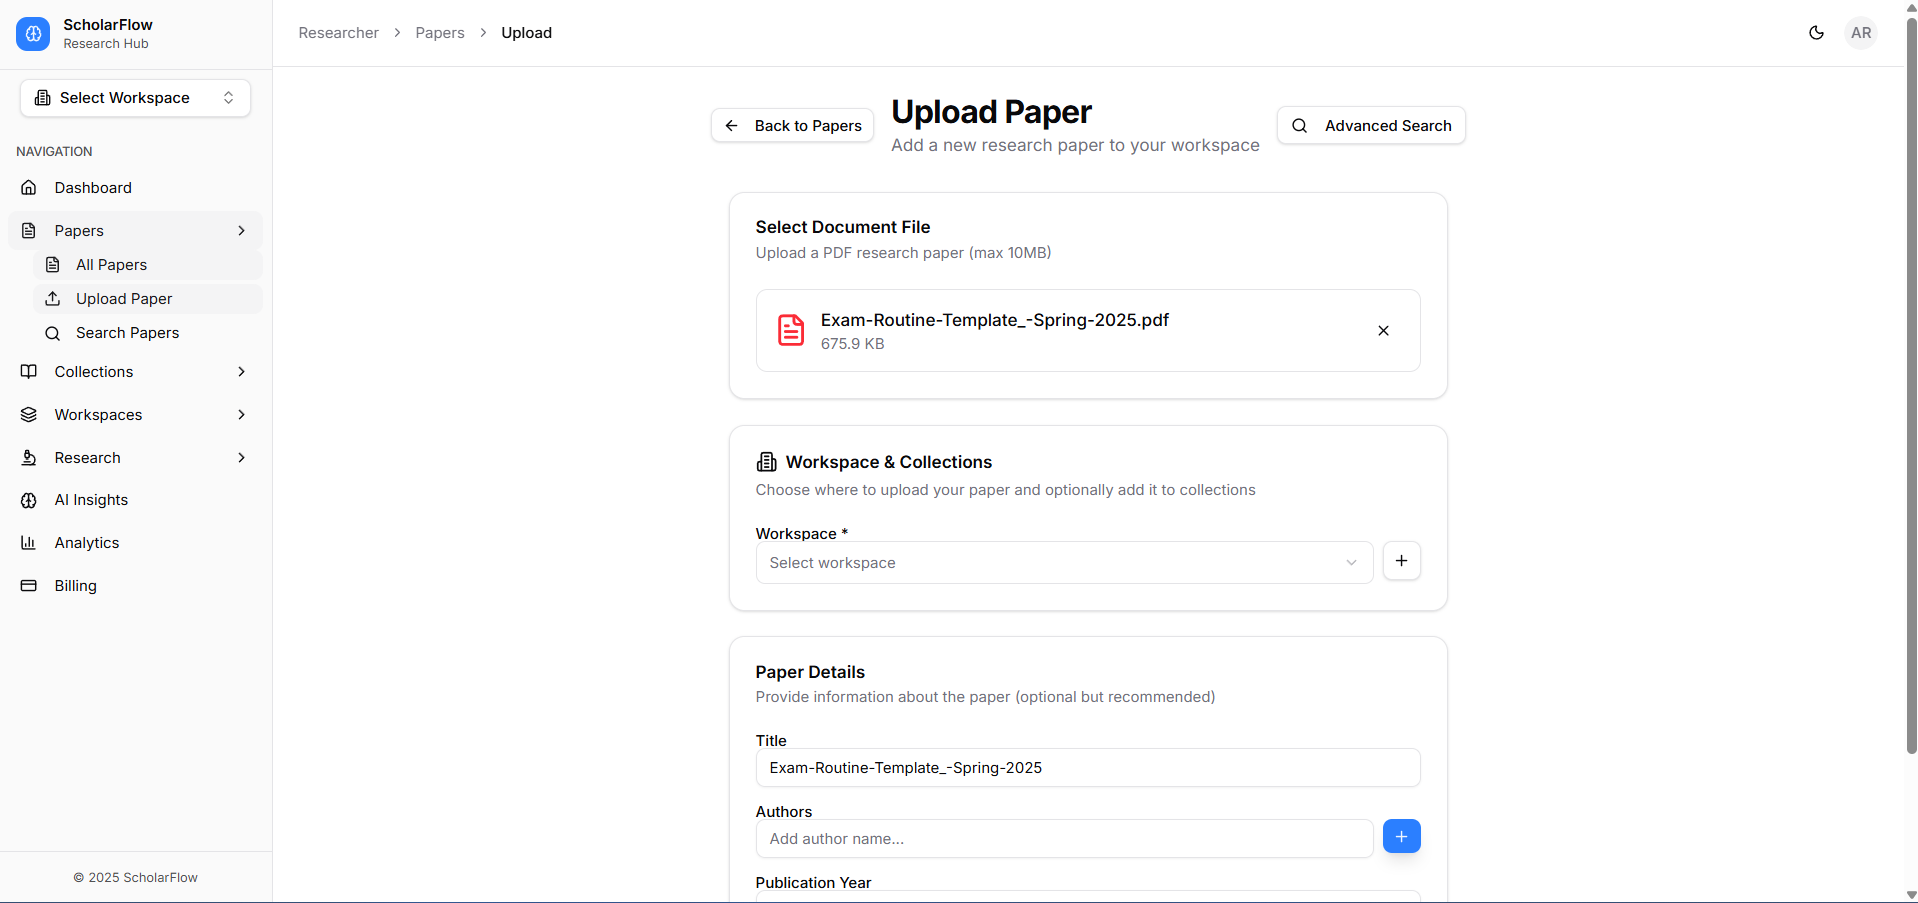
\includegraphics[width=0.75\textwidth]{images/screenshots/paper_upload.png}
\caption{Paper Upload Interface}
\label{fig:upload}
\end{figure}

\section{Advanced Search \& Filtering}

\textbf{Workflow:}
\begin{enumerate}[leftmargin=*,topsep=3pt,itemsep=2pt]
    \item User enters search query with optional filters (date range, author, type)
    \item Backend performs PostgreSQL full-text search using ILIKE operator
    \item Results ranked by relevance, paginated (20 per page)
    \item Metadata highlighted in results for quick identification
\end{enumerate}

\textbf{SQL Query:}
\begin{lstlisting}[language=SQL,basicstyle=\tiny\ttfamily]
SELECT p.id, p.title, p.abstract, p."createdAt"
FROM "Paper" p
WHERE p."workspaceId" = $1 AND p."isDeleted" = false
  AND (p.title ILIKE $2 OR p.abstract ILIKE $2)
ORDER BY p."createdAt" DESC LIMIT 20;
\end{lstlisting}

\begin{figure}[H]
\centering
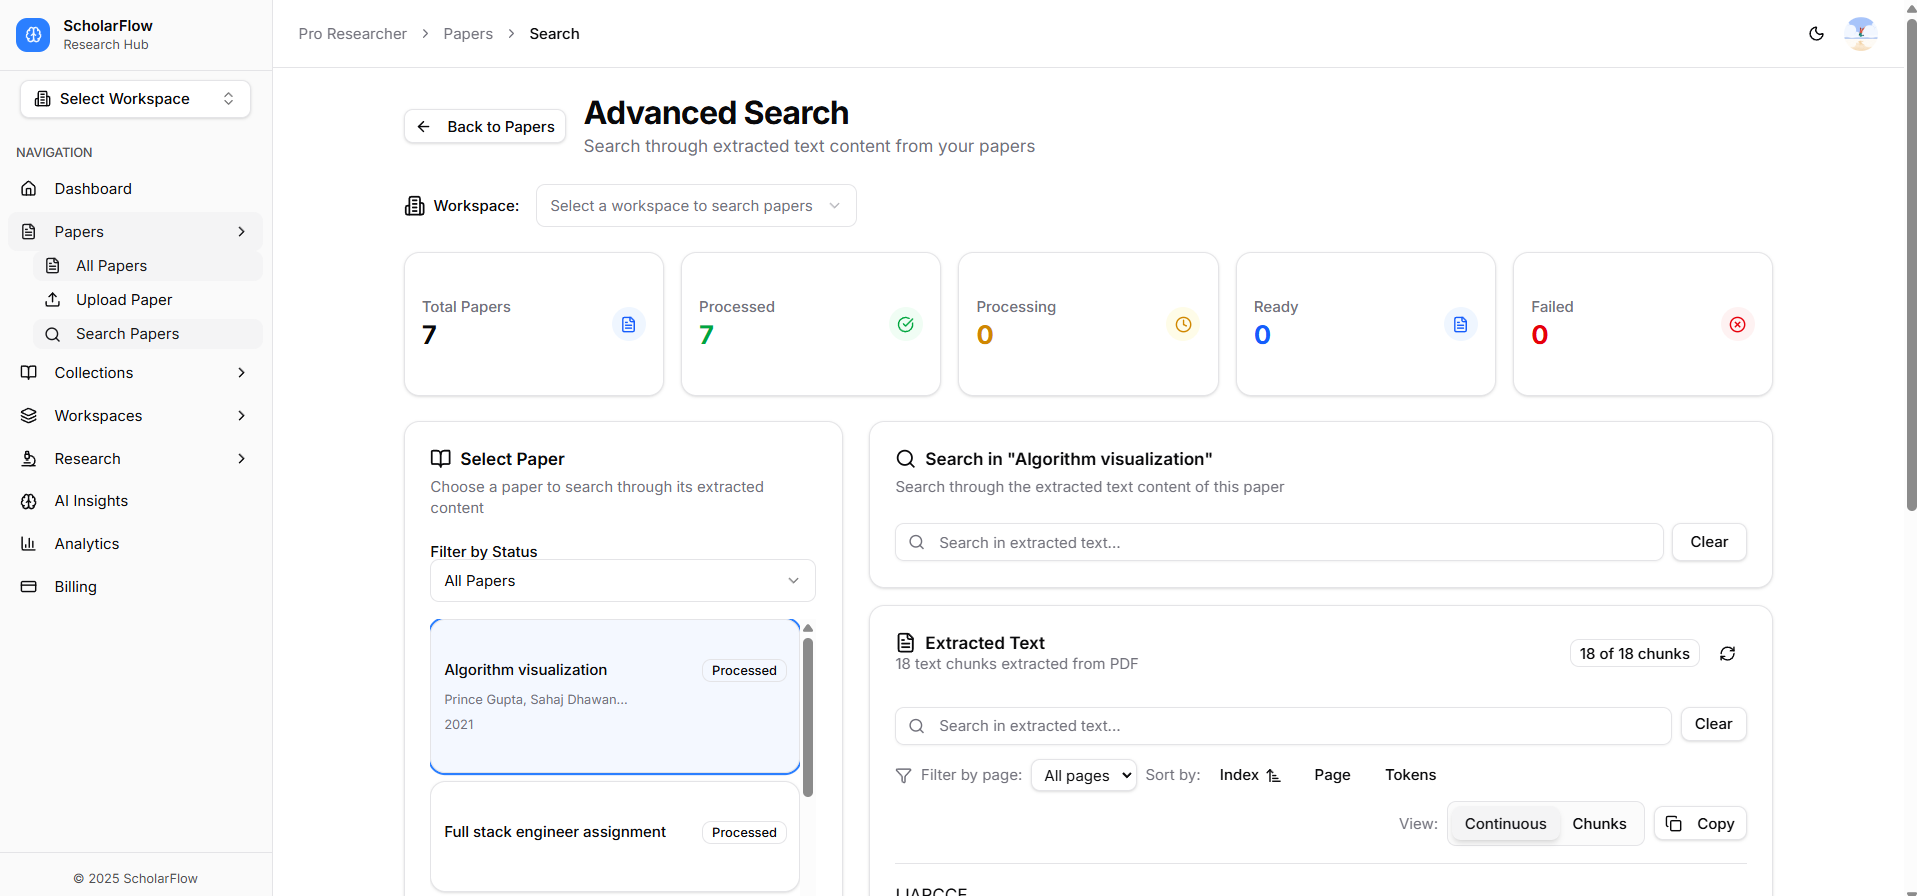
\includegraphics[width=0.8\textwidth]{images/screenshots/advanced_search.png}
\caption{Advanced Search Interface}
\label{fig:search}
\end{figure}

\section{Collection Management}

\textbf{Workflow:}
\begin{enumerate}[leftmargin=*,topsep=3pt,itemsep=2pt]
    \item User creates collection with name, description, privacy settings
    \item Papers added to collection via multi-select interface
    \item Collections shared with team members with role-based permissions (VIEW/EDIT)
    \item Members can view, add papers, or modify based on their role
\end{enumerate}

\textbf{Database Tables:} \texttt{Collection}, \texttt{CollectionPaper}, \texttt{CollectionMember}

\begin{figure}[H]
\centering
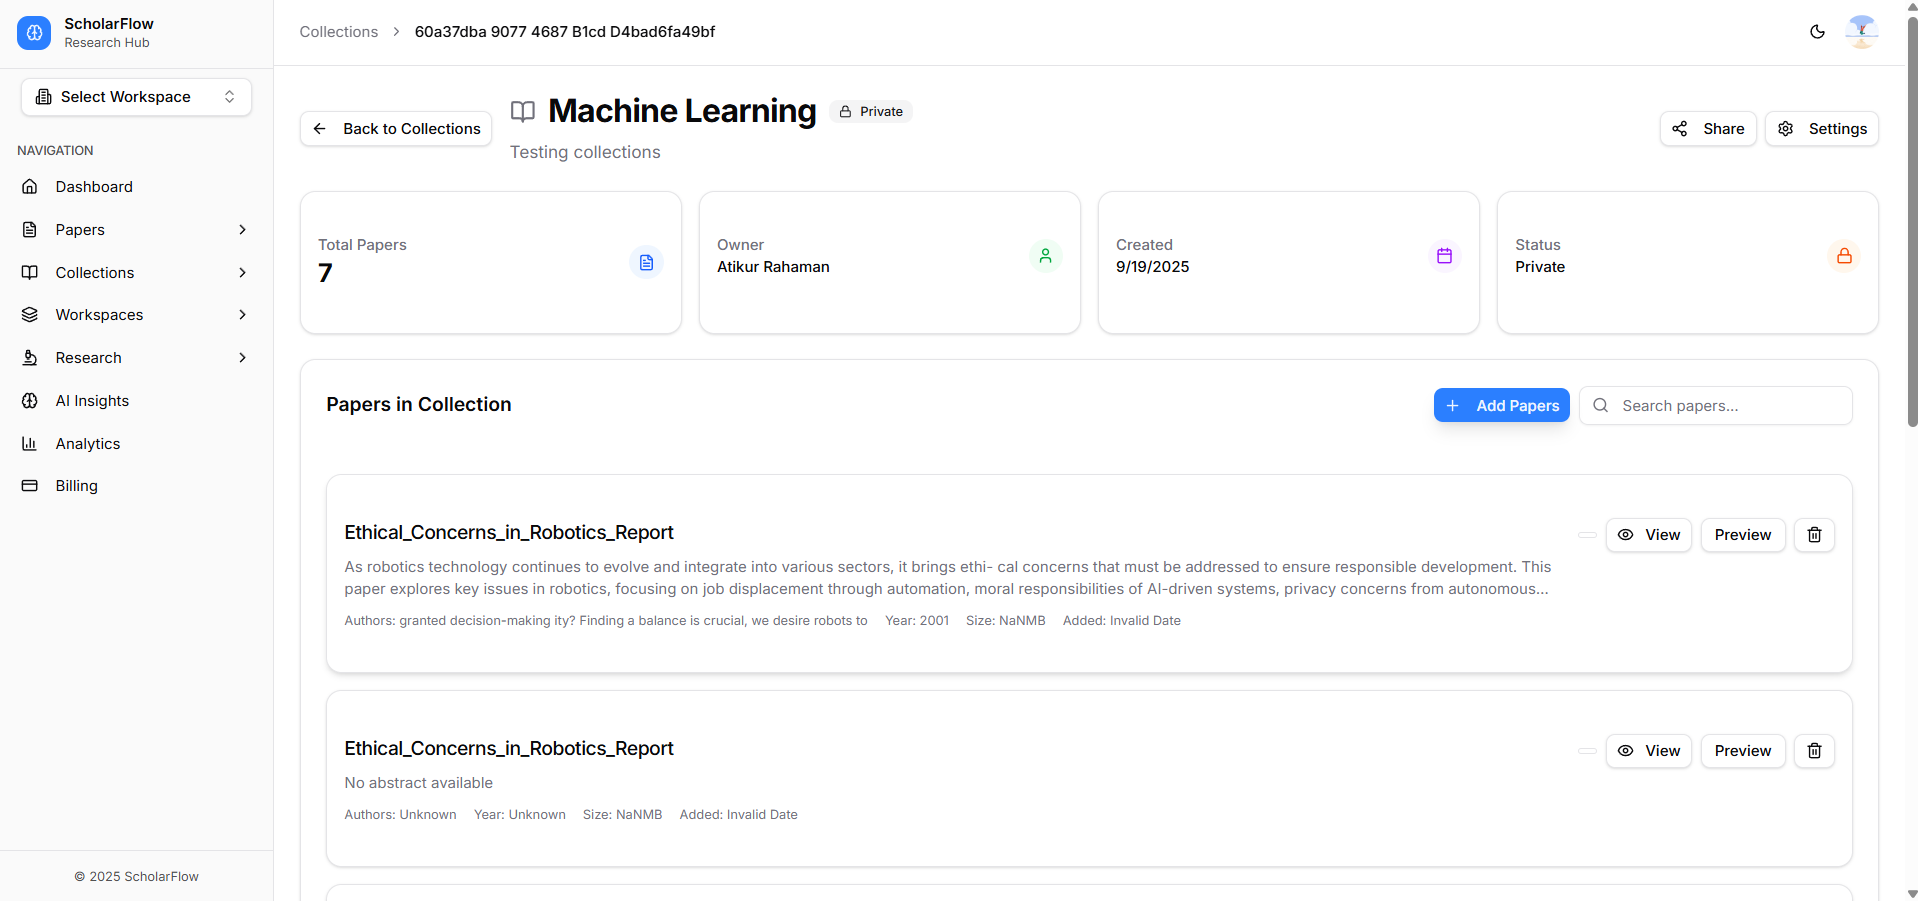
\includegraphics[width=0.75\textwidth]{images/screenshots/collection_details.png}
\caption{Collection Management}
\label{fig:collection}
\end{figure}

\section{AI-Powered Summarization \& Chat}

\textbf{Workflow:}
\begin{enumerate}[leftmargin=*,topsep=3pt,itemsep=2pt]
    \item User clicks "Generate Summary" on paper details page
    \item Backend retrieves paper chunks, sends to Gemini AI API
    \item AI generates concise summary highlighting key findings
    \item Summary cached in \texttt{AISummary} table for future access
    \item User can chat with paper, ask questions about content
\end{enumerate}

\textbf{Database Tables:} \texttt{AISummary}, \texttt{AIInsightThread}, \texttt{AIInsightMessage}

\begin{figure}[H]
\centering
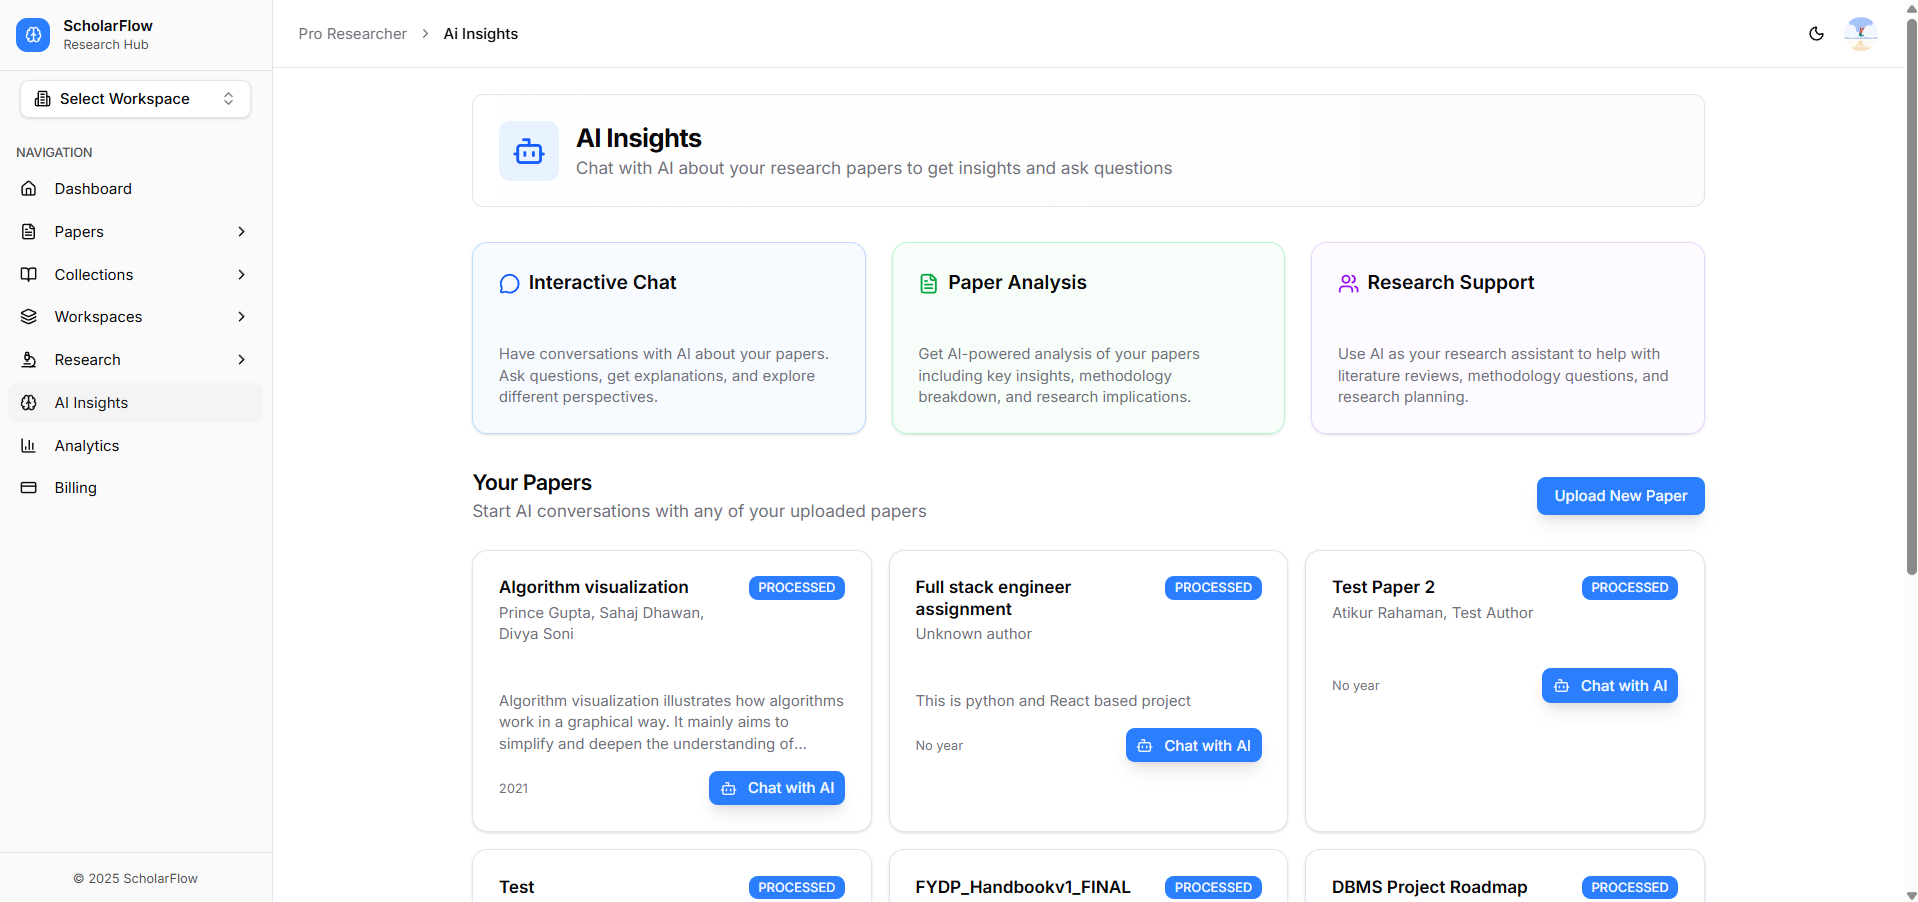
\includegraphics[width=0.8\textwidth]{images/screenshots/ai_insights.png}
\caption{AI Summary and Chat Interface}
\label{fig:ai}
\end{figure}

\section{Workspace Collaboration}

\textbf{Workflow:}
\begin{enumerate}[leftmargin=*,topsep=3pt,itemsep=2pt]
    \item Team lead creates workspace, invites members via email
    \item Invited users receive notification, accept invitation
    \item Members assigned roles: RESEARCHER, PRO\_RESEARCHER, TEAM\_LEAD, or OWNER
    \item Role determines permissions for paper upload, collection creation, member management
\end{enumerate}

\textbf{Database Tables:} \texttt{Workspace}, \texttt{WorkspaceMember}, \texttt{WorkspaceInvitation}

\begin{figure}[H]
\centering
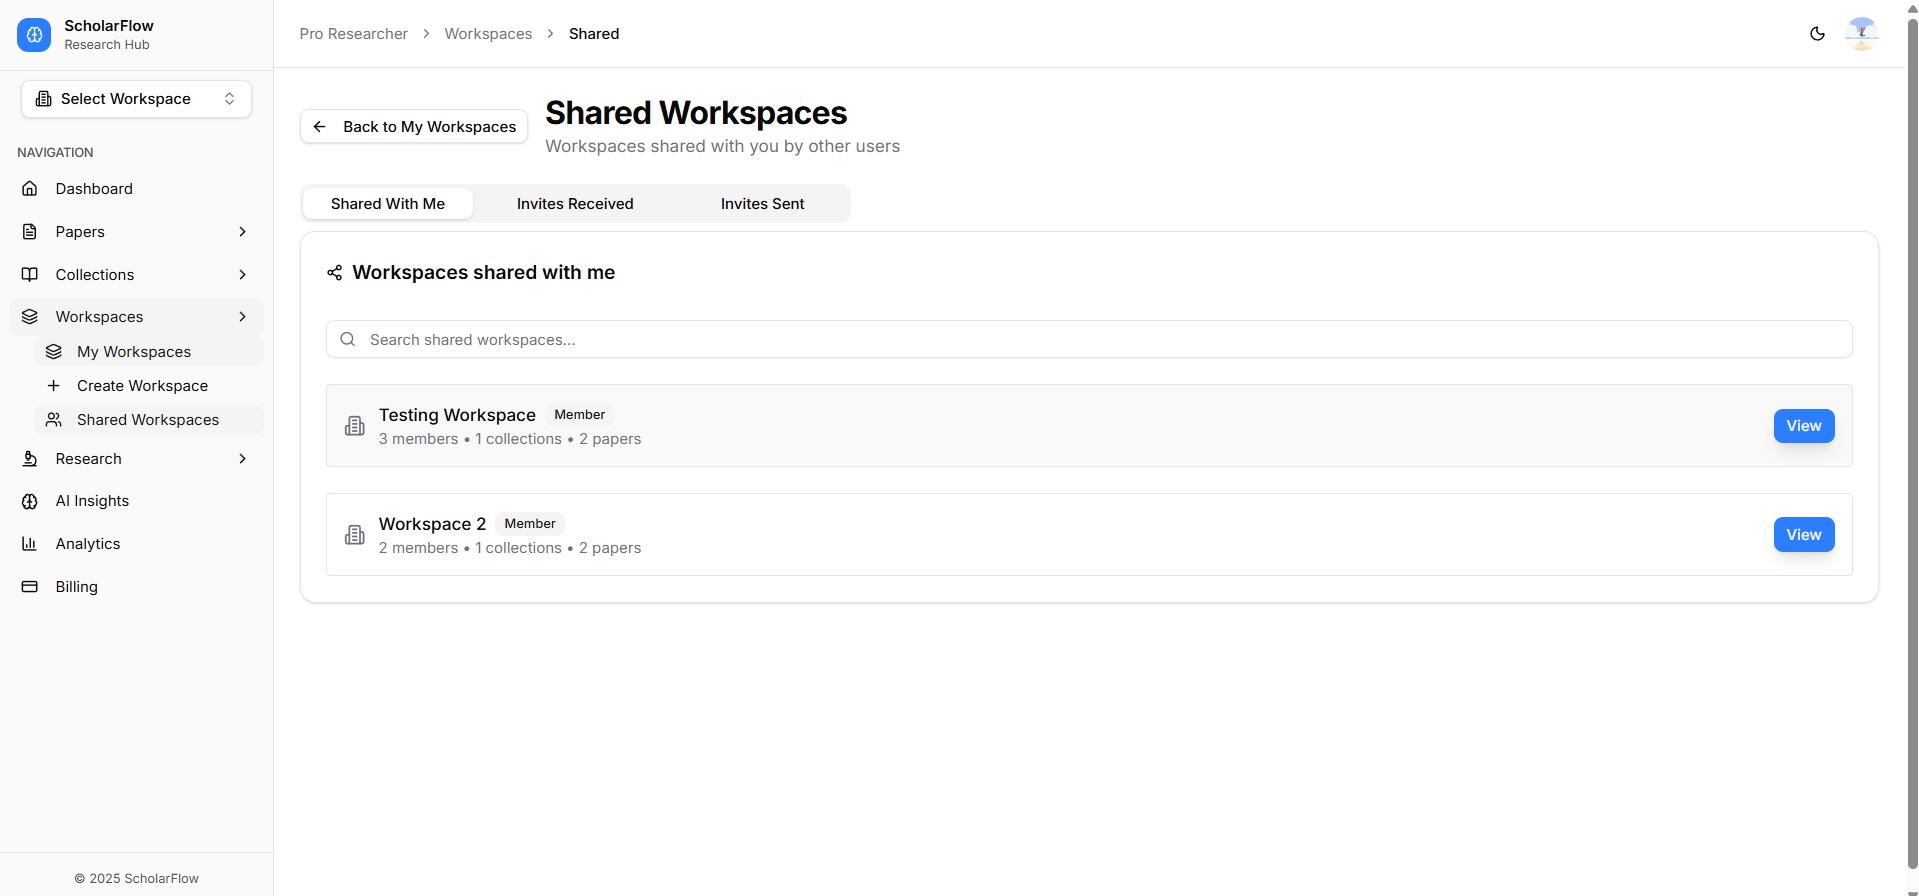
\includegraphics[width=0.75\textwidth]{images/screenshots/shared_workspace.png}
\caption{Workspace Collaboration Interface}
\label{fig:workspace}
\end{figure}

\section{Subscription \& Billing}

\textbf{Workflow:}
\begin{enumerate}[leftmargin=*,topsep=3pt,itemsep=2pt]
    \item User selects subscription plan (FREE, PRO, or INSTITUTIONAL)
    \item Redirected to Stripe Checkout for payment processing
    \item Stripe webhook confirms payment, updates user subscription status
    \item Subscription tracked in \texttt{Subscription} and \texttt{Payment} tables
    \item Users can manage subscription via Stripe Customer Portal
\end{enumerate}

\textbf{Database Tables:} \texttt{Subscription}, \texttt{Payment}, \texttt{UsageEvent}

\begin{figure}[H]
\centering
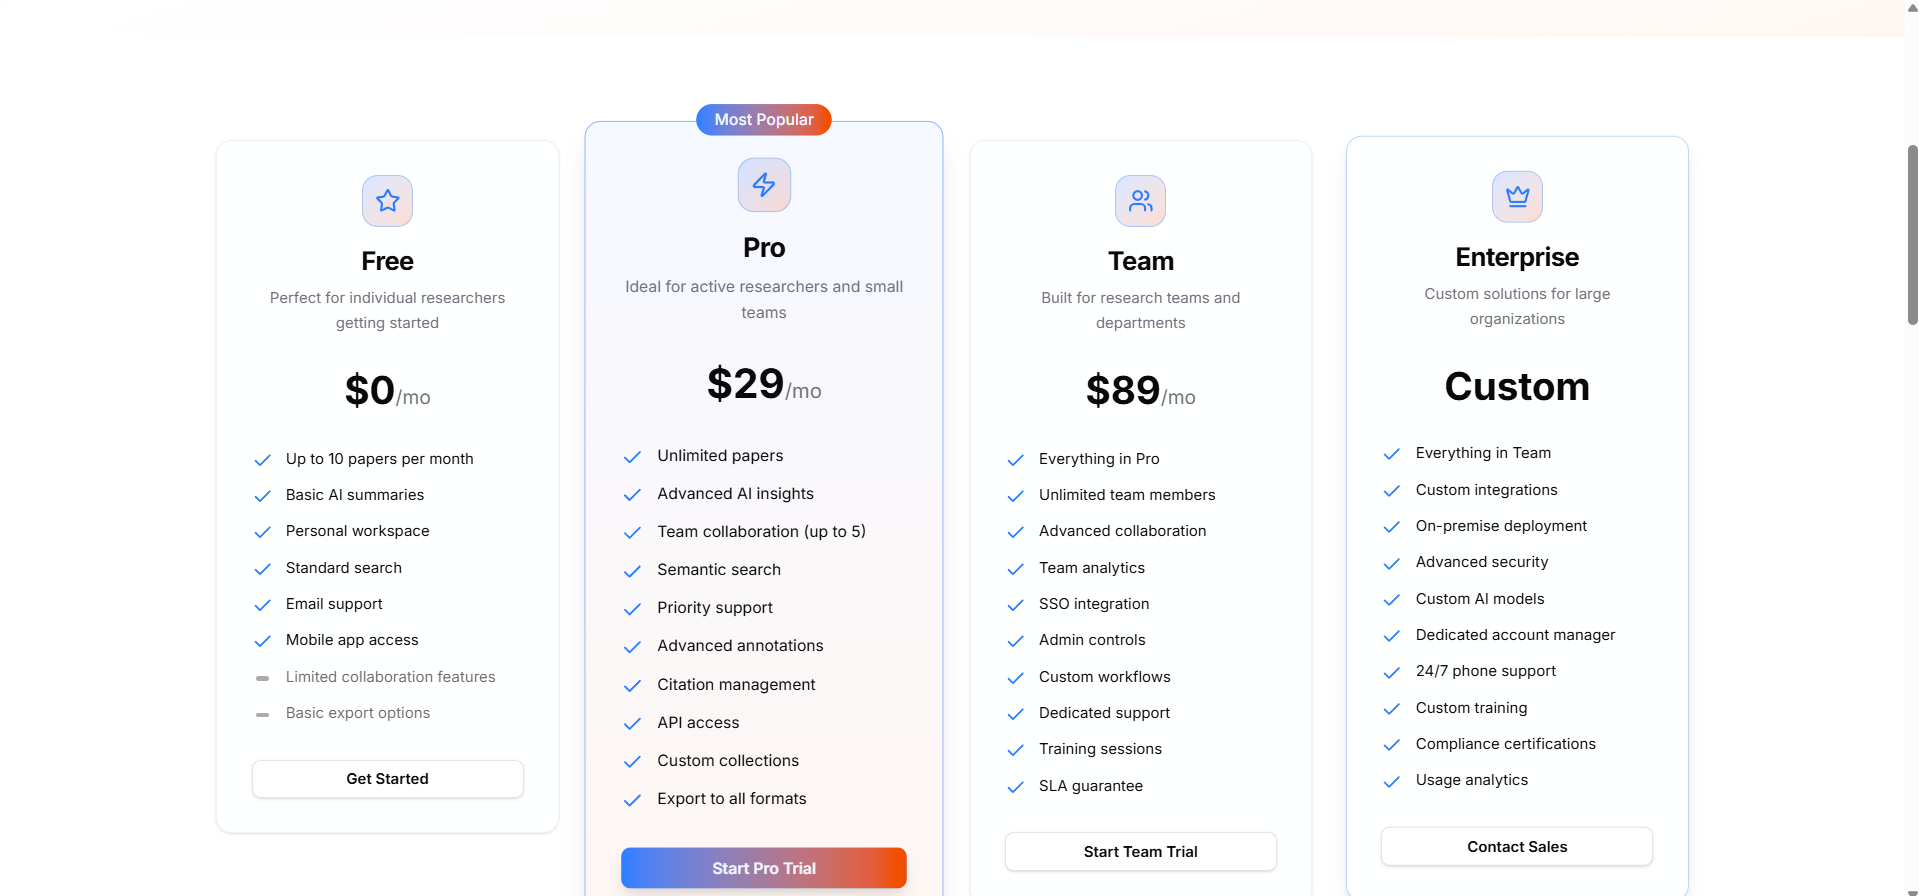
\includegraphics[width=0.7\textwidth]{images/screenshots/billing_plan.png}
\caption{Subscription Plans}
\label{fig:billing}
\end{figure}

\section{Admin Dashboard \& Analytics}

\textbf{Workflow:}
\begin{enumerate}[leftmargin=*,topsep=3pt,itemsep=2pt]
    \item Admin users access dashboard at \texttt{/admin} route
    \item Dashboard displays system metrics: total users, papers, active sessions
    \item Real-time health monitoring shows CPU, memory, database, storage status
    \item User management allows role changes, account suspension
    \item Analytics charts show user growth, paper uploads, revenue trends
\end{enumerate}

\textbf{Database Tables:} \texttt{User}, \texttt{Paper}, \texttt{Payment}, \texttt{ActivityLog}

\begin{figure}[H]
\centering
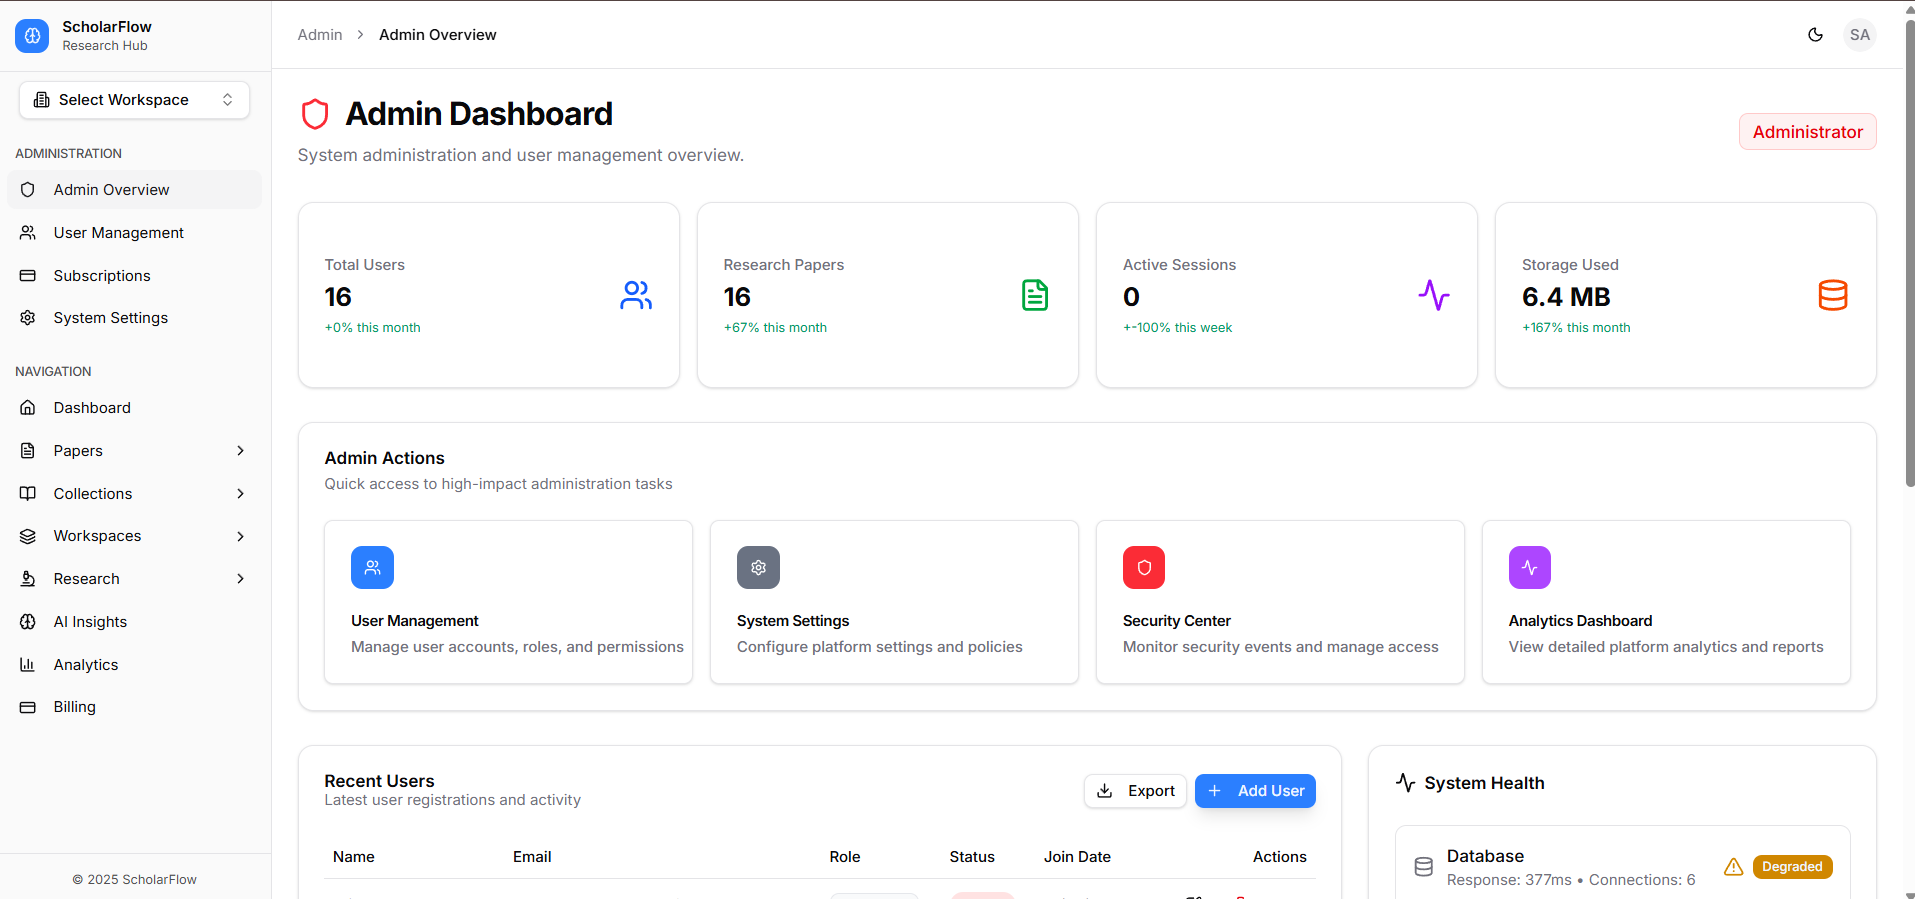
\includegraphics[width=0.85\textwidth]{images/screenshots/admin_overview.png}
\caption{Admin Dashboard}
\label{fig:admin}
\end{figure}

\section{Rich Text Editor with TipTap}

\textbf{Workflow:}
\begin{enumerate}[leftmargin=*,topsep=3pt,itemsep=2pt]
    \item User opens paper and clicks "Edit" to launch TipTap-based editor
    \item Complete toolbar with formatting: bold, italic, headings, lists, links, images
    \item Auto-save functionality with debounced updates every 2 seconds
    \item Image upload to S3 with drag-drop support and resizing capabilities
    \item Export notes to PDF/DOCX with embedded images and proper styling
    \item Share edited content via email with permission management
\end{enumerate}

\textbf{Database Tables:} \texttt{Paper}, \texttt{PaperContent}, \texttt{ActivityLog}

\begin{figure}[H]
\centering

\includegraphics[width=0.85\textwidth]{images/screenshots/text_editor.png}
\caption{Rich Text Editor Interface}
\label{fig:editor}
\end{figure}

\section{Research Notes \& Annotations}

\textbf{Workflow:}
\begin{enumerate}[leftmargin=*,topsep=3pt,itemsep=2pt]
    \item User creates structured research notes linked to papers
    \item Notes support markdown formatting, tags, and categorization
    \item Annotation system for highlighting and commenting on paper sections
    \item Notes are searchable across workspace with full-text indexing
    \item Export notes as PDF or markdown for external use
\end{enumerate}

\textbf{Database Tables:} \texttt{Note}, \texttt{Annotation}, \texttt{NoteTag}

\begin{figure}[H]
\centering
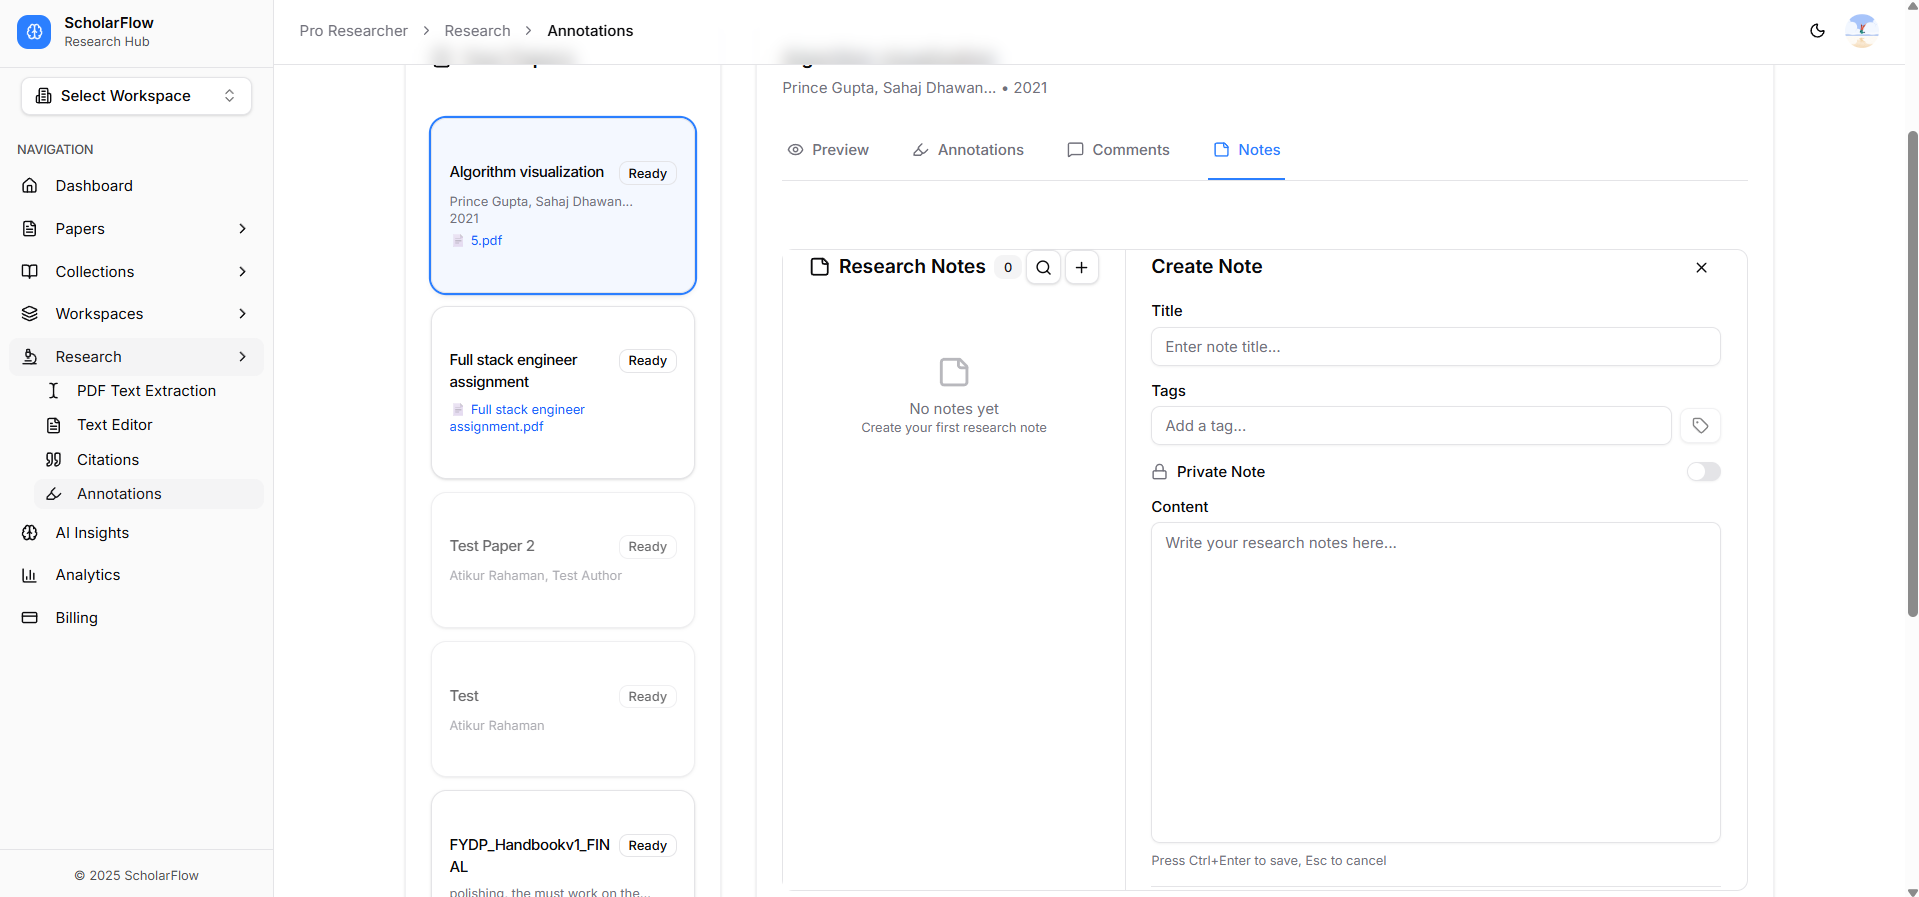
\includegraphics[width=0.8\textwidth]{images/screenshots/research_notes.png}
\caption{Research Notes Interface}
\label{fig:notes}
\end{figure}

\section{Citation Export \& Bibliography Management}

\textbf{Workflow:}
\begin{enumerate}[leftmargin=*,topsep=3pt,itemsep=2pt]
    \item User selects papers from workspace for citation export
    \item Choose format: BibTeX, RIS, EndNote, APA, MLA, or IEEE
    \item System generates formatted citations with complete metadata
    \item Export history tracked with download/delete functionality
    \item Direct copy-to-clipboard for quick citation insertion
\end{enumerate}

\textbf{Database Tables:} \texttt{Paper}, \texttt{CitationExport}, \texttt{ExportHistory}

\begin{figure}[H]
\centering
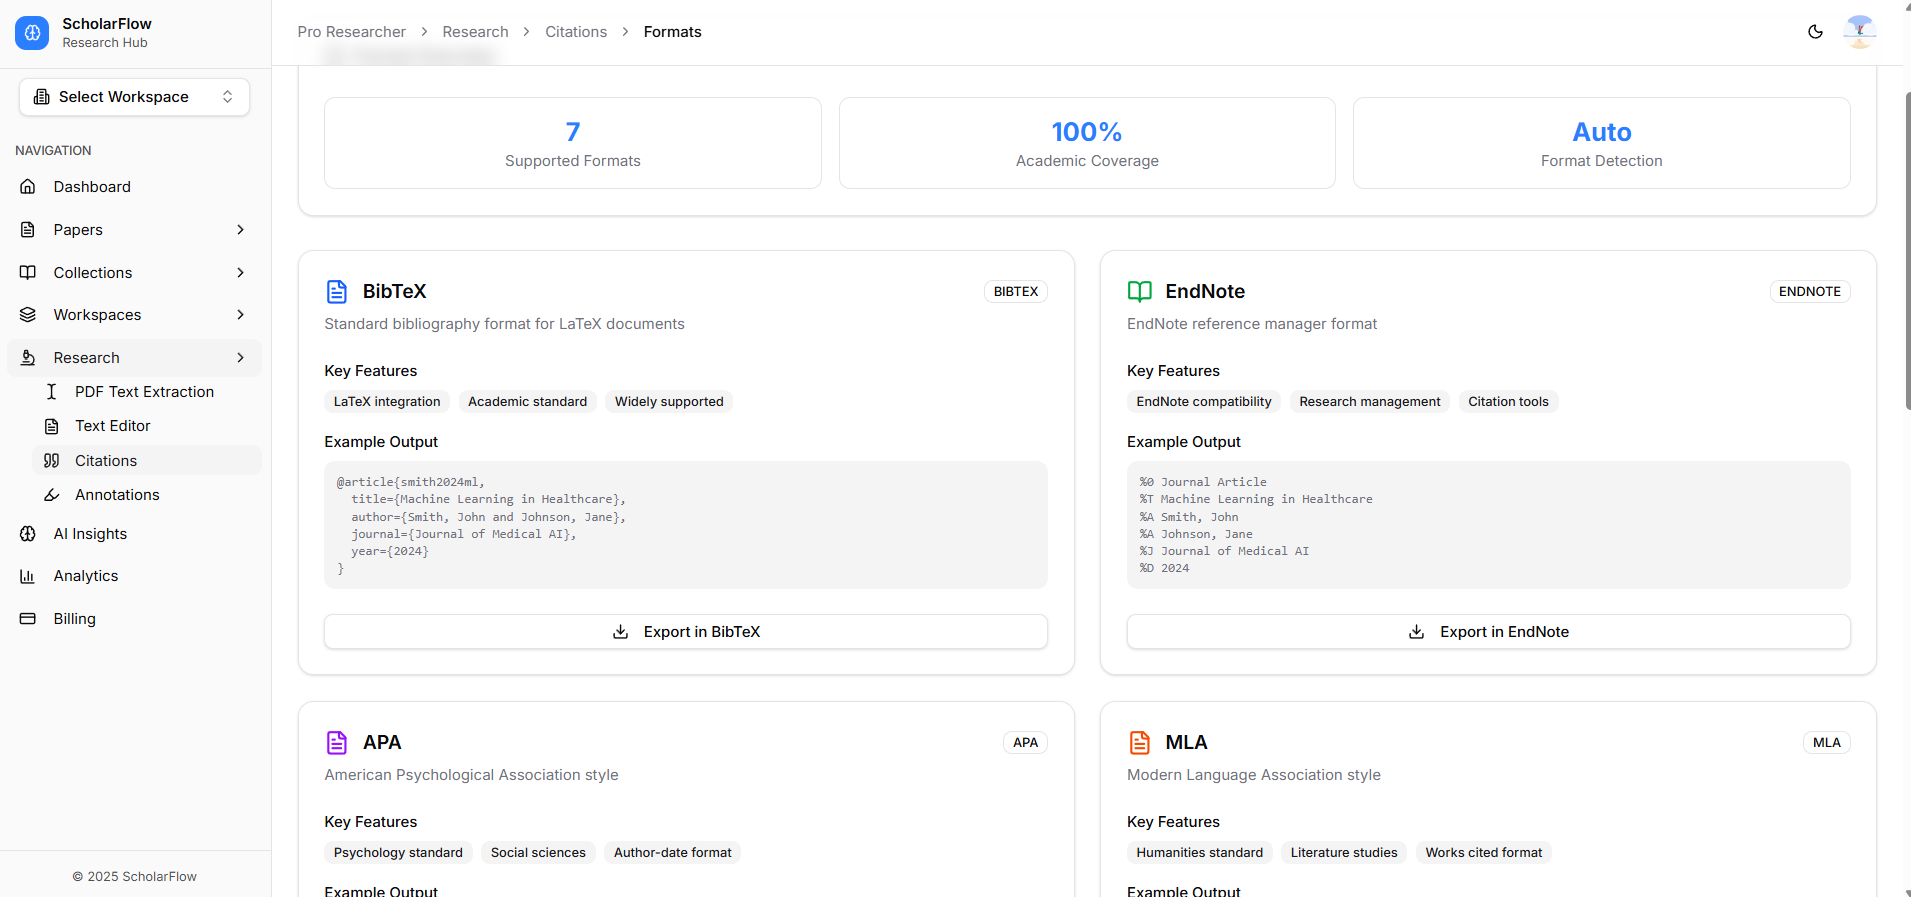
\includegraphics[width=0.8\textwidth]{images/screenshots/citations_formats.png}
\caption{Citation Export Formats}
\label{fig:citations}
\end{figure}

\section{Analytics Dashboard \& Insights}

\textbf{Workflow:}
\begin{enumerate}[leftmargin=*,topsep=3pt,itemsep=2pt]
    \item Dashboard displays workspace metrics: paper count, user activity, AI usage
    \item Interactive charts show paper uploads over time, collection growth
    \item Top contributors and most active users highlighted with engagement scores
    \item Export analytics reports for team performance tracking
    \item Real-time updates with refresh intervals configurable by user
\end{enumerate}

\textbf{Database Tables:} \texttt{ActivityLog}, \texttt{UsageEvent}, \texttt{AnalyticsSnapshot}

\begin{figure}[H]
\centering
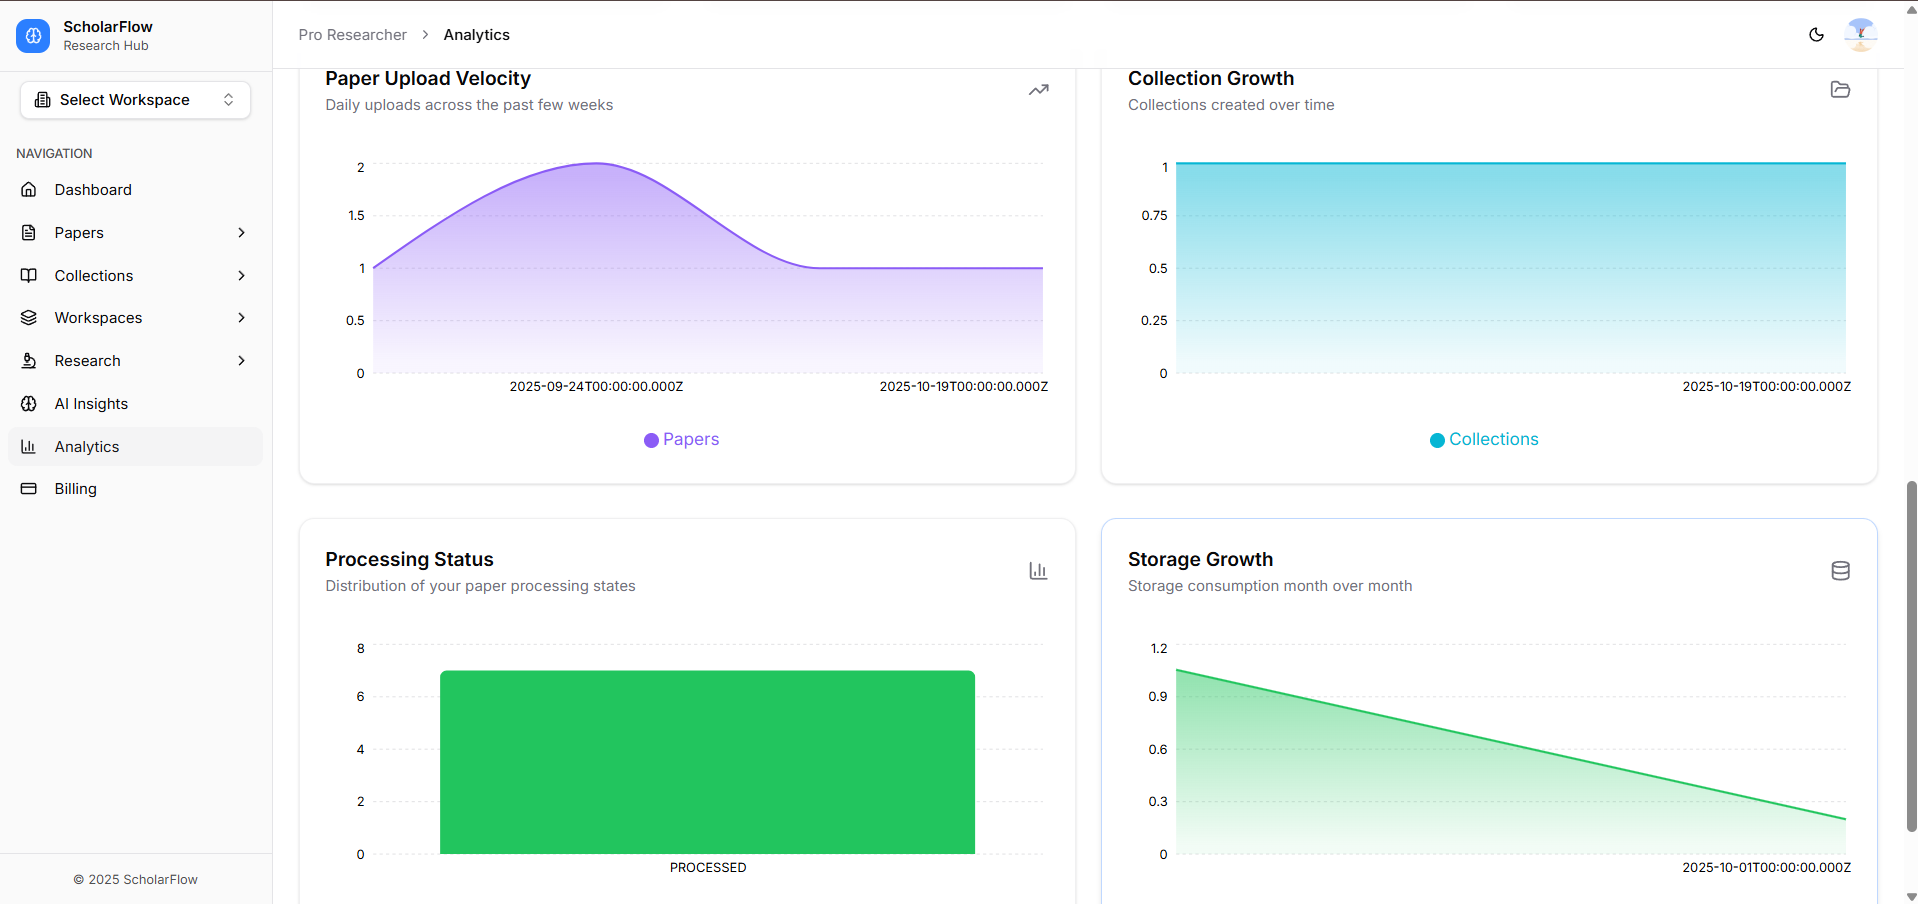
\includegraphics[width=0.85\textwidth]{images/screenshots/analytics.png}
\caption{Analytics Dashboard}
\label{fig:analytics}
\end{figure}

\section{System Health Monitoring}

\textbf{Workflow:}
\begin{enumerate}[leftmargin=*,topsep=3pt,itemsep=2pt]
    \item Admin dashboard displays real-time system health metrics
    \item Monitor CPU usage, memory consumption, database connections, storage
    \item Performance bars show resource utilization with color-coded status
    \item Automatic polling every 10 seconds with RTK Query caching
    \item Alert indicators for critical resource thresholds exceeded
\end{enumerate}

\textbf{Database Tables:} \texttt{SystemMetrics}, \texttt{HealthCheck}, \texttt{PerformanceLog}

\begin{figure}[H]
\centering
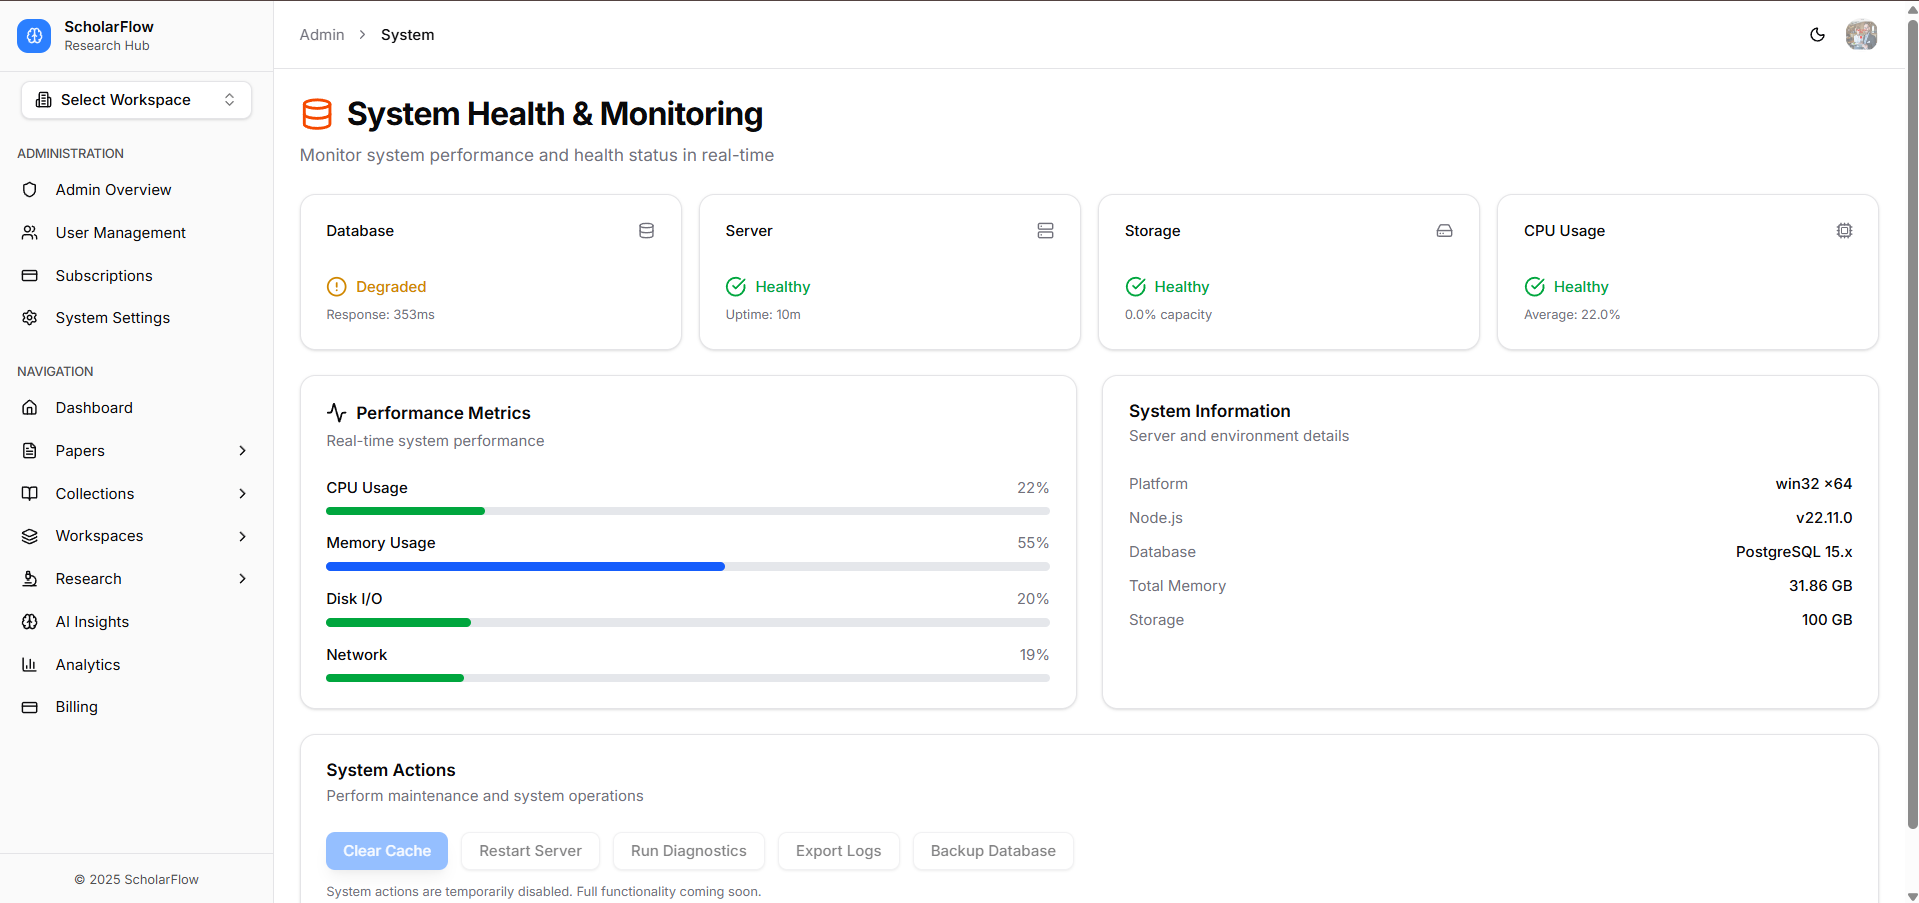
\includegraphics[width=0.85\textwidth]{images/screenshots/system_health.png}
\caption{System Health Monitor}
\label{fig:health}
\end{figure}
